\documentclass[11pt]{article}
\usepackage{amsmath, amssymb}
\usepackage{geometry}
\usepackage{graphicx}

% Set page margins
\geometry{margin=1in}

\title{Ordinary Differential Equations: \\ Separation of Variables and Initial Value Problems}
\author{Yang transcribed by Handwriting of Prof Langemann}
\date{07.11.2023}

\begin{document}

\maketitle

\section*{Introduction}
Ordinary differential equations (ODEs) are equations involving derivatives of a function. The solution of an ODE is the function itself. This handout will focus on the separation of variables technique and the consideration of initial value problems (IVPs).

\section*{2.1 Separation of Variables}
The separation of variables is a method to solve first-order ODEs that can be expressed as a product of two functions, one depending solely on the independent variable \( t \) and the other on the dependent variable \( y \).

\subsection*{Method}
Given an ODE in the form:
\[ y' = f(t,y) = g(t)h(y), \]
we can separate the variables and integrate both sides:
\[ \int \frac{1}{h(y)} \, dy = \int g(t) \, dt + C. \]

\subsection*{Example}
For the ODE \( y' = 2y/t \), we integrate both sides to find:
\[\frac{dy}{dt} = \frac{2y}{t}\]
\[ \int \frac{dy}{dt} = \int \frac{2y}{t} + C , C \in \mathbb{R}\]
which gives us the solution:
\[ ln|y| = 2ln|t| + C = ln t^2 + C\]
\[|y| = \pm e^c t^2\]
but \(y \equiv 0\) is also a solution

\subsection*{Remarks}
Care is required when solving the integrals, especially when the ODE is autonomous (only dependent on \( y \)).

\subsection*{Autonomous ODEs}
Autonomous ODEs are time-independent and can be expressed as \( y' = f(y) \). They often have solutions that can be visualized as a family of curves representing different trajectories based on initial conditions.

\section*{Initial Value Problems (IVPs)}
According **Frobenius’ Theorem:** Addresses the existence and uniqueness of the solution to an ODE given an initial condition \( y(t_0) = y_0 \).

\subsection*{**Unique Solution:** }
If \( t \neq 0 \) and \( y_0 \neq 0 \), there is a unique solution through the point \( (t_0, y_0) \).

\subsection*{**Multiple Solutions:** }
If \( y_0 = 0 \), there may be multiple solutions, including the trivial solution \( y = 0 \).

\subsection*{**No Solution:** }
Under certain conditions, there may be no solution that satisfies the initial value problem.

\subsection*{Conclusion}
The separation of variables is a powerful technique for solving first-order ODEs. It is particularly useful when the ODE can be separated into a function of \( t \) and a function of \( y \). The consideration of initial conditions is crucial for determining the uniqueness and existence of solutions to an ODE.
\section*{The Example}
Given the differential equation:
\[ y' = 1 - 2y \]

The direction field can be sketched and the following separation of variables can be performed:

\begin{align*}
\frac{dy}{dt} &= 1 - 2y \\
\int \frac{dy}{1 - 2y} &= \int dt + c \\
\frac{1}{-2} \ln |1 - 2y| &= t + c \\
|1 - 2y| &= e^{-2c} \cdot e^{-2t} \\
1 - 2y &= \pm e^{-2c} \cdot e^{-2t} && \text{(assuming $y = \frac{1}{2}$ at $t=0$)} \\
y &= \frac{1}{2}(1 - C e^{-2t}), \quad c \in \mathbb{R}
\end{align*}

The particular solution given the initial condition \( y = \frac{1}{2} \) at \( t = 0 \) is:
\[ y = \frac{1}{2}(1 - C e^{-2t}) \]



Considering the substitution \( y' = \frac{dy}{dt} \) , \(\eta = y(\tau)\)and the differential equation:
\[ y(t) - y_0 =\int_{y_0}^{y(t)}d\tau = \int_{t_0}^{t} y'(\tau) \, d\tau \]
which implies:
\[ \int_{y_0}^{y(t)} \frac{dy}{g(y)} = \int_{t_0}^{t} f(t,y(t)) \, dt \]

Using discretization, we define \( \Delta y_i = y_{i+1} - y_i \) and approximate:
\[ \int_{y_0}^{y(t)} 1dy \approx \sum_{i=0}^{n-1} \Delta y_i \approx \sum_{i=0}^{n-1} f(t_i,y_i) \Delta t_i \approx 
\int_{t_0}^{t} f (\tau. y(\tau))d\tau\]


We consider the product-type approximation:
\[ f(t_i,y_i) \approx g(t_i) \cdot h(y_i) \]
and
\[ \frac{\Delta y_i}{\Delta t_i} \approx g(t_i) \cdot h(y_i) or \frac{\Delta y_i}{h(y_i)} \approx g(t_i) \Delta t_i\]

Then, in the limit as \( n \rightarrow \infty \), we get:
\begin{align*}
\int_{y_0}^{y(t)} \frac{dy}{h(\eta)} &= \lim_{n \rightarrow \infty \& \Delta y_i \rightarrow 0} \sum_{i=0}^{n-1} \frac{\Delta y_i}{g(t_i,y_i)} \\
&\approx \lim_{n \rightarrow \infty} \sum_{i=0}^{n-1} g(t_i) \Delta t_i = \int_{t_0}^{t} g(\tau) \, d\tau
\end{align*}




Consider the differential equation:
\[ y' = \sqrt{1 - y^2} \]
and the frequent situation:
\[ y' = -a(t)y \]

For the first equation, we show the stages in the recipe of separation of variables:
\begin{align*}
\frac{dy}{dt} &= \sqrt{1 - y^2} \\
\int \frac{dy}{\sqrt{1 - y^2}} &= \int dt + c \\
\arcsin(y) &= t + c \\
y(t) &= \sin(t + c)
\end{align*}

However, the last line marked as "Wrong" suggests a misconception in the solution process.

For the frequent situation, the process is:
\begin{align*}
\frac{dy}{dt} &= -a(t)y \\
\int \frac{1}{y} dy &= -\int a(t) dt + c \\
\ln |\frac{y(t)}{y_0}| &=  \int_{t_0}^{t} a(\tau) d\tau + c \\
|\frac{y(t)}{y_0}| &= - e^{\int_{t_0}^{t} a(\tau) d\tau}\\
y(t) &= y_0\cdot e^{-\int a(\tau) d\tau}
\end{align*}

It is also noted that solutions never pass \( y = 0 \) as shown in the sketch.

\subsection{}section*{Remark}
The sketch includes a direction field for \( y' = \sqrt{1 - y^2} \), indicating regions where \( y' \geq 0 \) and \( y(t) \) is monotonically increasing, as well as a phase line analysis showing that solutions are confined within \( -1 < y < 1 \) and never reach the values \( y = \pm 1 \).


\subsection*{Matrix Version}

For the vector function \(\mathbf{q}(t)\), consider the differential equation in matrix form:
\[ \mathbf{q}' = -A(t) \mathbf{q} \]
with \( A(t) \in \mathbb{R}^{n \times n} \).

The solution can be expressed as:
\[ \mathbf{q}(t) = e^{-\int_{t_0}^{t} A(\tau) d\tau} \cdot \mathbf{q}_0 \]
where \( \mathbf{q}_0 \in \mathbb{R}^n \).

This involves the matrix exponential:
\[ e^B = \sum_{k=0}^{\infty} \frac{B^k}{k!} = I + B + \frac{B^2}{2!} + \ldots \]
where \( B \in \mathbb{R}^{n \times n} \) and \( I \) is the identity matrix.


\section*{2.2 DEs in Homogeneous Variables}

\textbf{Definition:} A homogeneous function \( f = f(t,y) \) of degree \( n \) is such that:
\[ f(\lambda t, \lambda y) = \lambda^n f(t,y) \]

For example, for \( n = 0 \):
\[ f(\lambda t, \lambda y) = f(1, \frac{y}{t}) = g(\frac{y}{t}) \]
where \( f \) depends only on \( \frac{y}{t} \).

\textbf{Ingredient:}
\[ y' = g\left(\frac{y}{t}\right) \]
i.e., the right-hand side is homogeneous of degree 0.

\textbf{Recipe:}
Substitute \( u = \frac{y}{t} \) i.e., \( y = u \cdot t \).

Then:
\[ y' = u' \cdot t + u \]
Thus:
\[ u' \cdot t + u = g(u) \]
or equivalently:
\[ u' = \frac{1}{t} (g(u) - u) \tag{*} \]

\textbf{Result (\(*\)):} Use 2.1.

\textbf{Example:}
\[ y' = \frac{t - y}{t + y} = \frac{1}{1 + \frac{y}{t}} = \frac{1}{1 + u} \]
Substituting \( u = \frac{y}{t} \) we have:
\[ u' \cdot t + u = \frac{1}{1 - u} \]
i.e.,
\[ u' = \frac{1}{t} \left(\frac{1}{1 - u} - u\right) = \frac{1 - u + u^2}{t(1 - u)} \]


\subsection*{Separation of Variables}

Performing separation of variables and applying partial fraction decomposition (PFD), we get:
\[
\int \frac{1-u}{1-u+u^2} \, du = \int \frac{dt}{t} + c
\]

\newpage
\date{15.11.2023}
\subsection*{ODE}



\section*{2.3 Linear Differential Equation of First Order}

A linear differential equation of the form:
\[
y' + a(t)y = P(t)
\]
where \( P(t) \) is the external excitation on the right-hand side. The corresponding homogeneous equation is:
\[
y' + a(t)y = 0
\]
and the inhomogeneous equation is:
\[
y' + a(t)y = P(t) \neq 0
\]

\subsection*{Recipe}
To solve the inhomogeneous ODE:
\begin{enumerate}
    \item Solve the homogeneous ODE \( y_h = C y_t \), with arbitrary factor \( C \in \mathbb{R} \).
    \item Solve the inhomogeneous ODE by variation of the constant \( C \) to get one particular solution \( y_p \).
\end{enumerate}
The general solution is:
\[
y = y_p + C y_t, \quad C \in \mathbb{R}
\]
because of the linearity property \( \mathcal{L}\{y_p + C y_t\} = \mathcal{L}\{y_p\} + C \cdot 0 = P \).

\subsection*{Comparison to Linear Algebra}
For an operator \( \mathcal{L} \) analogous to matrix \( A \) in \( \mathbb{R}^{n \times n} \) with rank \( A = n-1 \), the kernel \( \ker(A) = \{ x \in \mathbb{R}^n \mid Ax = 0 \} \) has dimension 1. That is, the solution space \( x_h = C x_t \).

For a particular solution \( A x_p = b \), the general solution is \( x = x_p + C x_t \).

\subsection*{Example}
For \( A \in \mathbb{R}^{2 \times 2} \), \( A = \begin{pmatrix} 1 & 1 \\ 2 & 2 \end{pmatrix} \) with rank \( A = 1 \), and \( A \begin{pmatrix} x \\ y \end{pmatrix} = \begin{pmatrix} b_1 \\ b_2 \end{pmatrix} \), the kernel of \( A \), \( \ker(A) \), and the particular solution \( x_p \) are computed as follows:

The kernel \( \ker(A) = \{ x \in \mathbb{R}^2 \mid Ax = 0 \} \) is the line of multiples of \( x_t = (-c, c) \).

The particular solution \( x_p = \begin{pmatrix} \frac{1}{2} \\ \frac{1}{2} \end{pmatrix} \) with \( A x_p = b \) is shown in the diagram.

\begin{figure}[h!]
\centering
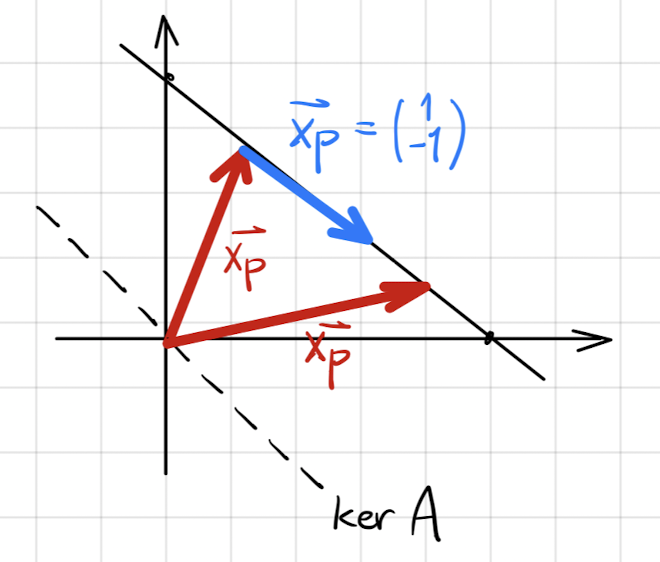
\includegraphics[width=0.5\textwidth]{solution_space.png}
\caption{Diagram showing the solution space with \( x_p \) and \( \ker(A) \).}
\end{figure}



\section*{Some Concepts from Linear Algebra}

Consider a matrix \( A \) defined as:
\[ A = \begin{pmatrix}
    a_{11} & \cdots & a_{1m} \\
    \vdots & \ddots & \vdots \\
    a_{n1} & \cdots & a_{nm}
\end{pmatrix} \in \mathbb{R}^{n \times m} \]

This matrix maps \( \mathbb{R}^m \) to \( \mathbb{R}^n \) by:
\[ \vec{x} = \begin{pmatrix}
    x_1 \\
    \vdots \\
    x_m
\end{pmatrix} \quad \text{such that} \quad A\vec{x} \]

A system of linear equations is given by \( A\vec{x} = \vec{b} \).

\subsection*{Example}
For the system
\[ \begin{pmatrix}
    1 & 1 \\
    3 & 4
\end{pmatrix} \begin{pmatrix}
    x_1 \\
    x_2
\end{pmatrix} = \begin{pmatrix}
    5 \\
    17
\end{pmatrix} \]
we have a unique solution space. The solution is
\[ \begin{pmatrix}
    x_1 \\
    x_2
\end{pmatrix} = \begin{pmatrix}
    3 \\
    2
\end{pmatrix} \]

For the system
\[ \begin{pmatrix}
    1 & 1 \\
    3 & 3
\end{pmatrix} \begin{pmatrix}
    x_1 \\
    x_2
\end{pmatrix} = \begin{pmatrix}
    5 \\
    14
\end{pmatrix} \]
there is no solution.

However, with
\[ \begin{pmatrix}
    1 & 1 \\
    3 & 3
\end{pmatrix} \begin{pmatrix}
    x_1 \\
    x_2
\end{pmatrix} = \begin{pmatrix}
    5 \\
    15
\end{pmatrix} \]
and \( A\vec{x} \neq \vec{0} \), we have a space of solutions.

\subsection*{Space of Solution}
The set
\[ M = \left\{ \begin{pmatrix}
    x_1 \\
    x_2
\end{pmatrix} = \begin{pmatrix}
    5 \\
    0
\end{pmatrix} + c \begin{pmatrix}
    1 \\
    -1
\end{pmatrix} \right\} \in \mathbb{R}^2 \]
includes \( \vec{x}_p \) (particular solution) and \( \vec{x}_t \) (trivial solution).

\subsection*{Kernel of A}
The kernel of \( A \) is defined as:
\[ \ker(A) = \left\{ \vec{x} \mid A\vec{x} = \vec{0} \right\} \]

\subsection*{Example}
The kernel of a differential operator \( \frac{d}{dt} \) is a constant function since the derivative of a constant is 0, hence the dimension of the kernel is 1.

\subsection*{Image of A}
The image of \( A \) is defined as:
\[ \text{im}(A) = \left\{ \vec{y} \mid A\vec{x} = \vec{y} \right\} \]



\section*{Solution of First-Order Linear ODE}

\subsection*{Homogeneous Equation}
For the homogeneous equation
\[ \frac{dy}{dt} = -a(t)y \]
we find the integrating factor \( \mu(t) \) such that
\[ \mu(t) = e^{-\int a(t) \, dt} \]
and the solution of the homogeneous equation is
\[ y_h = C \cdot \mu(t) \]
where \( C \) is an arbitrary constant.

\subsection*{Variation of the Constant}
The particular solution \( y_p \) can be found by letting \( C(t) \) be a function of \( t \):
\[ y_p = C(t) \cdot \mu(t) \]
Substitute into the ODE to find \( C(t) \) as follows:
\begin{align*}
C(t) \mu(t) + C'(t) \mu(t) y_t + a(t) C(t) \mu(t) &= P(t) \\
C'(t) \mu(t) &= P(t) \\
C(t) &= \int \frac{P(t)}{\mu(t)} \, dt
\end{align*}
The general solution of the ODE is:
\[ y = y_h + y_p = \mu(t) \left( C + \int \frac{P(t)}{\mu(t)} \, dt \right) \]

\subsection*{Example}
For the differential equation
\[ y' + 2y = 1 \]
\begin{enumerate}
    \item The homogeneous part \( y' + 2y = 0 \) has the solution \( y_h = C e^{-2t} \).
    \item For the inhomogeneous part with external excitation, we find \( y_p \) by:
    \[ y_p = C(t) e^{-2t} \]
    and by differentiating \( y_p \) and substituting into the ODE, we get \( C(t) \) and therefore \( y_p \).
\end{enumerate}
The general solution of the ODE is:
\[ y = y_p + C y_h = \frac{1}{2} + C e^{-2t}, \quad C \in \mathbb{R} \]



\section*{Example: Differential Equation with Periodic External Excitation}

Consider the differential equation
\[ y' + y = \sin(\alpha t) \]
with periodic external excitation. For the homogeneous equation \( y_h = C e^{-t} \), where \( C \in \mathbb{R} \), we have a transient solution \( y_t = e^{-t} \).

\subsection*{Particular Solution}
For the particular solution \( y_p \), let \( y_p = C(t)e^{-t} \), and find \( C(t) \) as follows:
\[ y_p' = C'(t)e^{-t} - C(t)e^{-t} \]
Substituting into the differential equation gives
\[ C(t) = \int e^{t} \sin(\alpha t) \, dt = \frac{\sin(\alpha t) - \alpha \cos(\alpha t)}{1 + \alpha^2} e^{-t} \]
Thus, the particular solution becomes
\[ y_p = \frac{\sin(\alpha t) - \alpha \cos(\alpha t)}{1 + \alpha^2} \]
with the system response in phase with the excitation frequency \( \alpha \).

Using trigonometric identities, we can express \( y_p \) as
\[ A \sin(\alpha t - \varphi) = A \sin \alpha t \cos \varphi + A \cos \alpha t \sin \varphi \]
where
\[ A \cos \varphi = \frac{1}{1 + \alpha^2}, \quad A \sin \varphi = \frac{\alpha}{1 + \alpha^2} \]
and thus
\[ A^2 = \frac{1}{(1 + \alpha^2)^2} + \frac{\alpha^2}{(1 + \alpha^2)^2} = \frac{1}{1 + \alpha^2} \]
giving us
\[ \tan \varphi = \alpha \]

\begin{figure}[h!]
\centering
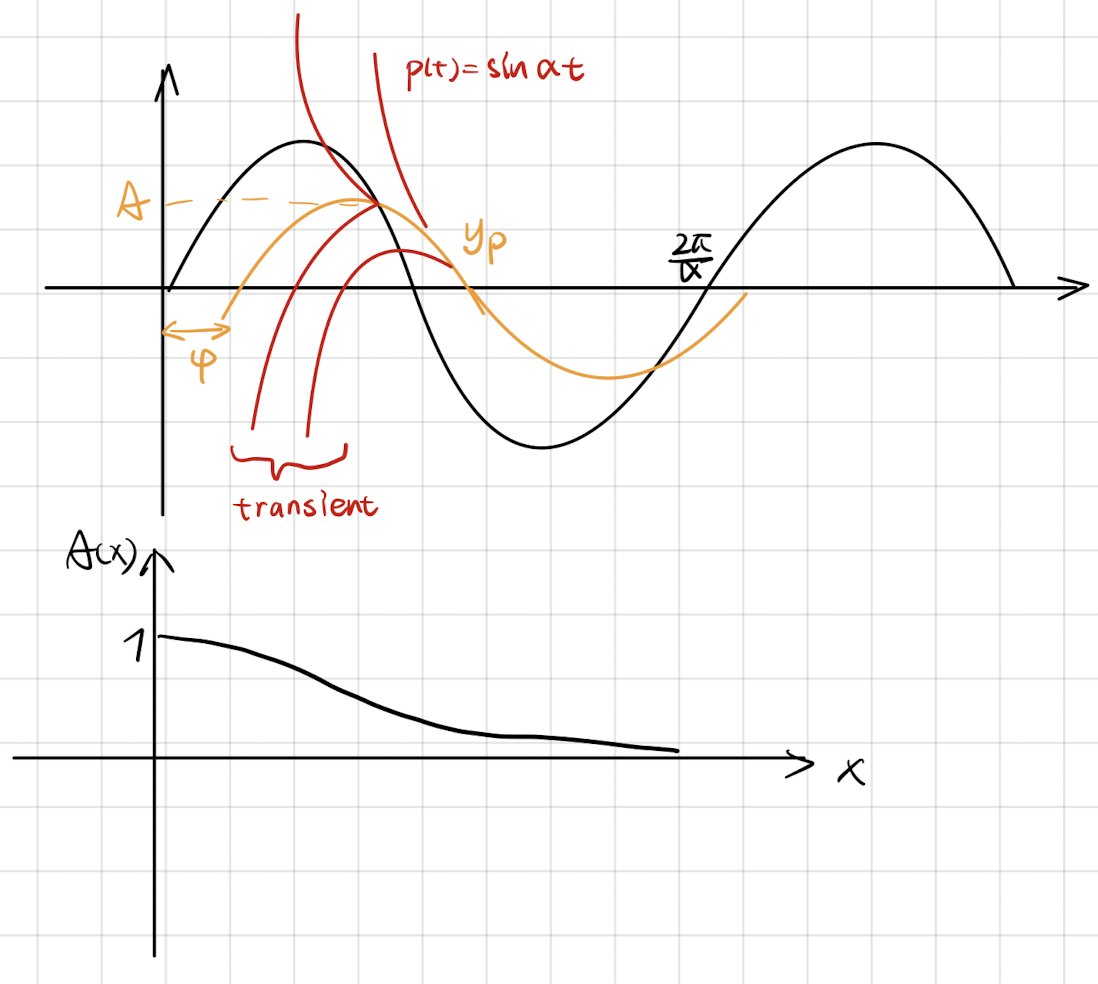
\includegraphics[width=0.5\textwidth]{response_curve.png}
\caption{Response curve showing the transient and steady-state parts of the solution.}
\end{figure}

\section*{2.4 Bernoulli's Differential Equation}
Bernoulli's ODE of the form
\[ y' + a(t)y = p(t)y^n, \quad \text{where } n \neq 0,1 \]
can be solved by the substitution \( u = y^{1-n} \), which yields
\[ u' + (1-n)a(t)u = (1-n)p(t) \]
This transforms the Bernoulli's ODE into a linear ODE, which can be solved using the methods described in section 2.3.


\section*{Example: Logistic Growth}

Consider the logistic growth differential equation:
\[ y' = y(1-y) \]

This can be rearranged to:
\[ y' = y - y^2 \]

Using the substitution \( u = \frac{1}{y} \), we get:
\[ u' = -\frac{y'}{y^2} \]

Substituting the original equation, we have:
\[ -u' = u - 1 \]
or equivalently
\[ u' = 1 - u \]

The solution is:
\[ u = 1 + Ce^{-t}, \quad C \in \mathbb{R} \]

Back substituting to find \( y \), we get:
\[ y = \frac{1}{1 + Ce^{-t}}, \quad C \in \mathbb{R} \]

\begin{figure}[h!]
\centering
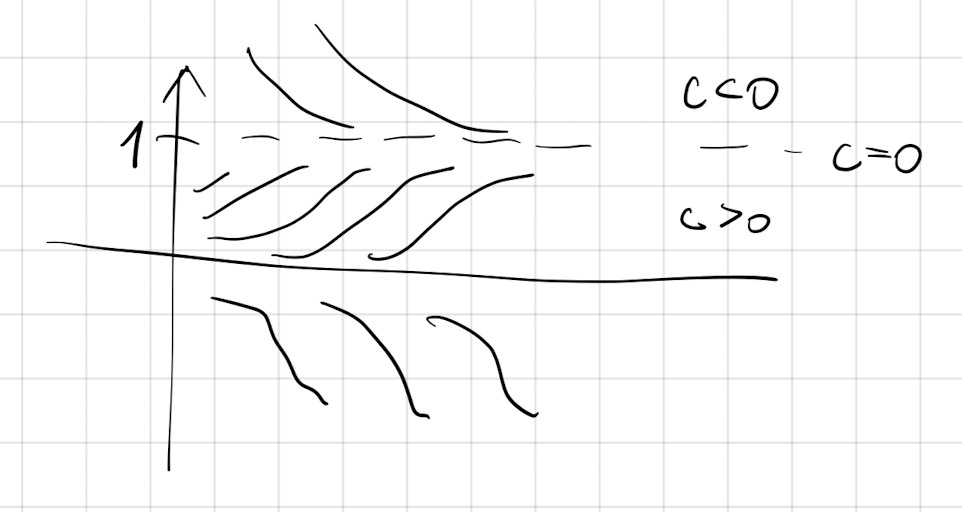
\includegraphics[width=0.5\textwidth]{phase_diagram.png}
\caption{Phase diagram for the logistic growth equation.}
\end{figure}

\end{document}
